\documentclass[../main.tex]{subfiles}
\begin{document}
\chapter{Avionics Protocols}
\label{chap:avionicsprot}

Avionics telecomunications have undergone a major upgrade in the last years
which is still in progress as new standards are set to be fully deployed within
the next decade. Such changes are made to bring the benefits of modern tecnology
onboard of the aircrafts and in the \textbf{Air Traffic Management}
(\textbf{ATM}) world.

Different organizations collaborate in defining the standards and guidance
documents for aeronautics, the major are the Radio Technical Commission for
Aeronautics (\textbf{RTCA}) in the United States, the European Organisation for
Civil Aviation Equipment (\textbf{EUROCAE}) in Europe and the International
Civil Aviation Organization (\textbf{ICAO}) which is United Nations
organization. All this organizations are non governative therefore they produce
standards, guidelines or rules that will then have to be adopted by the Federal
Aviation Administration (\textbf{FAA}) in the united states, by the
\textbf{EUROCONTROL}\footnote{Organization to provide unique centralized
platform for civil and military aviation coordination in Europe.} and the single
national aviation autority of the various european countries
(\textit{ENAC/ENAV}\footnote{Ente Nazionale Aviazione Civile e Ente Nazionale
Assistenza Volo} in Italy). This fragmentation of the organizations, the
absence of a global shared guidance on the standardization of the aviation
sector (which is partially an \textbf{ICAO} task.\footnote{Art 1. The
contracting States recognize that every  State has complete and exclusive
sovereignty over the airspace above its territory.\cite{icao7300}}) and the
developement of different standards to acomplish the same task brought to an
unclear situation regarding standards and regulations, for this reasons some
problems in the the definition of a globally accepted NextGen family of
protocols rose in the latest years; this will be discussed in the appropriate
section.

\todo{something more}

There are two way of identifying an aircraft:
\begin{itemize}
  \item The classic radar (or Primary Radar), based on electromagnetic waves which is only able to give information on a position of an object in the sky. Such system gives a real-time image of the portion of sky that it is observing, this includes aircrafts, birds, clouds, and any other object in his field of view making it a basic and farely unreliable system. Since this method requires no interaction with the aircraft that is beeing traced it is called \textbf{non-cooperative} system.
  \item Second Surveillance Radar (SSR) is an evolution of the above system which, in addition to the spatial position of the aricraft, requests additional information depending on his mode of operation. Since this system requires an active cooperation from the aircraft which must reply to the information requests send by the system it is called \textbf{cooperative} system.
\end{itemize}

Cooperative systems allow to have a bidirectional aircraft-ground as well as aircraft-aircraft data flow. This system stems from the military Identification Friend or Foe (\textbf{IFF}) one which was developed during the second World War. The actual civil system uses a 4 digit code called "Transponder Code" or \textbf{"Squawk"} to identify the aircraft, this communicates via a \textbf{transponder} which handles the incoming interrogations and the responses. In Figure \ref{fig:allgen} is an overview of all the protocols and their division between the old generation and the new generation which is still in deployiment.

\begin{figure}[htp]
  \centering
  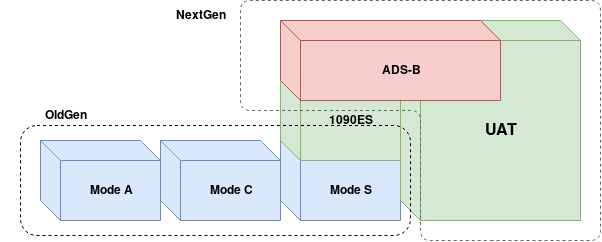
\includegraphics[scale=0.6]{images/allgen.png}
  \caption{All generation of avionics protocols}
  \label{fig:allgen}
\end{figure}

Having a continuous data flow between the aircraft and the groud has many benefits:
\begin{itemize}
  \item Flight controllers can obtain much more information about a single aircraft, his intentions, the status of the flight and real time weather information from the onboard sensors. Moreover satellite based ADS-B allows tracing aircrafts in areas where no radar coverage is available (e.g. over the ocean).
  \item The airline can keep track of his fleet in real time thus allowing a better planning of the turnover and quick deployiment of replacement aeroplane.
  \item The maintenance branch of the airline can track in real time any anomalies reported by the aircraft instruments and sensors performing a remote analysis and helping the pilots in the troubleshooting process helping them to take better decisions.
\end{itemize}

% \begin{figure}[htp]
%   \centering
%   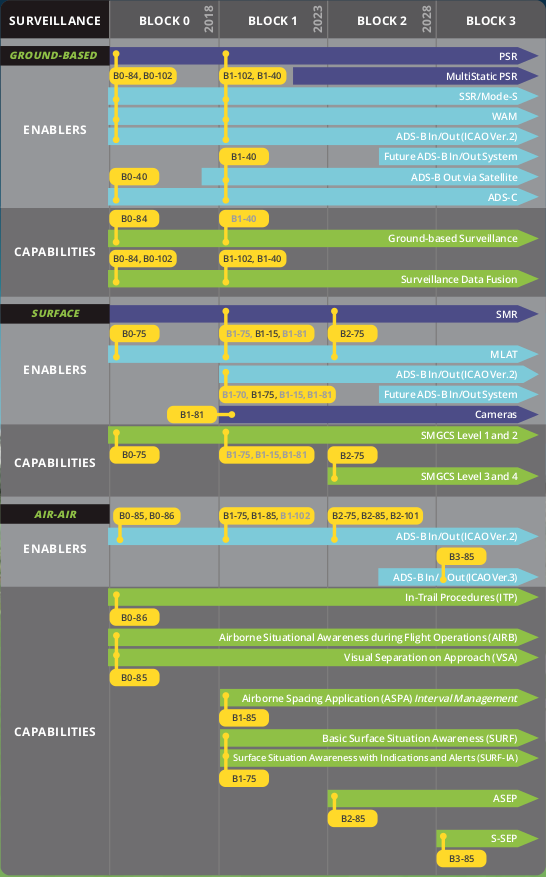
\includegraphics[scale=0.85]{images/survmode.png}
%   \caption{}
%   \label{}
% \end{figure}

\section{OldGen}
\todo{acars messages. explain how 1090mhz/1030MHZ protocols works.}

The first generation of protocols is fairly simple, it uses the 1030MHz frequency for interrogation while the 1090MHz frequency is used for replies.
The first two protocols are \textbf{Mode A} and \textbf{Mode C}.

\textbf{Mode A} is the simplest, it responds to an interrogation request just by broadcasting the \textbf{squawk} code which was previously assigned to the pilot by the controller. In this way the controller can identify the aircrafts on his screen by such code. In addition to this the pilot can manually generate a special response called \textit{"Ident"} which is used to highlight the aircraft on the controller screen\footnote{\ask{Tecnical specifications of such response are defined in ICAO Annex 10 Volume IV.}}.
\todo{images of the signal???}

\textbf{Mode C} is an extention of the previous protocol which, in addition to the transponder code, sends information about the altitude and the pressure. This kind of transponders are often referred as \textbf{Mode A/C} transponder.

\textbf{Mode S} is the newest protocol and it is an hybrid between the two generations. It is backward compatible with the \textbf{Mode A/C} but at the same time it is also part of the NextGen as it can be seen in Figure \ref{fig:allgen}. 

\todo{ads-b/ads-c in between old and next or actually is in both}

\section{NextGen}

\todo{explain how 978/nexrad/tis-b/fis-b protocols works}
\todo{The American Federal Aviation Administration (FAA) as
well as its European EUROCONTROL named ADS-
B as the satellite-based successor of radar.}
\todo{maybe explain backwards compatibility with 1090 using 1090ES (extended squitter) also put the theory about using fis-b/tis-b in uat and 1090mhz band. (Find some references and obtain some documents FREE)}

\todo{Where mode-ac and mode-s are used now}

\end{document}
